\documentclass{article}
\usepackage[utf8]{inputenc}
\usepackage{graphicx}
\usepackage{amsmath}
\usepackage{hyperref}
\usepackage{booktabs}
\usepackage{float}

\title{Análisis Estadístico de un Dataset}
\author{Tu Nombre}
\date{\today}

\begin{document}

\maketitle

\tableofcontents
\newpage

% --- Sección 1: Introducción ---
\section{Introducción}
\subsection{Contexto del Problema}
Breve descripción del contexto y los objetivos del análisis. ¿Por qué es importante este dataset? ¿Qué preguntas se buscan responder?

\subsection{Descripción del Dataset}
Información general sobre el dataset:
\begin{itemize}
    \item Fuente de los datos.
    \item Número de filas y columnas.
    \item Variables principales y su tipo (numérica, categórica, etc.).
\end{itemize}

% --- Sección 2: Análisis Exploratorio de Datos (EDA) ---
\section{Análisis Exploratorio de Datos (EDA)}
\subsection{Limpieza de Datos}
\begin{itemize}
    \item Manejo de valores faltantes.
    \item Tratamiento de outliers.
    \item Corrección de inconsistencias.
\end{itemize}

\subsection{Análisis Descriptivo}
    \subsubsection{Estadísticas descriptivas (media, mediana, desviación estándar, etc.).}


\begin{table}[H]
    \centering
    \begin{tabular}{|l|r|}
    \hline
    \textbf{Estadística} & \textbf{Valor} \\
    \hline
    Duración Media & 99.528 \\
    Duración Mediana & 98.000 \\
    Moda de la Duración & 90.000 \\
    Varianza (min$^2$) & 804.816 \\
    Desviación Estándar & 28.369 \\
    Percentil 25 & 87.000 \\
    Percentil 50 (mediana) & 98.000 \\
    Percentil 75 & 114.000 \\
    \hline
    \end{tabular}
    \caption{Duración de Películas}
    \label{tab:estadisticas_duracion_peliculas}
\end{table}

\begin{table}[H]
    \centering
    \begin{tabular}{|l|r|}
    \hline
    \textbf{Estadística} & \textbf{Valor} \\
    \hline
    Duración Media & 1.765 \\
    Duración Mediana & 1.000 \\
    Moda de la Duración & 1.000 \\
    Varianza (\#temporadas$^2$) & 2.505 \\
    Desviación Estándar & 1.583 \\
    Percentil 25 & 1.000 \\
    Percentil 50 (mediana) & 1.000 \\
    Percentil 75 & 2.000 \\
    \hline
    \end{tabular}
    \caption{Duración de Series de TV}
    \label{tab:estadisticas_duracion_series}
\end{table}

\begin{table}[H]
    \centering
    \begin{tabular}{|l|r|}
    \hline
    \textbf{Estadística} & \textbf{Valor} \\
    \hline
    Mediana & 2017 \\
    Moda & 2018 \\
    Varianza & 78 \\
    Desviación Estándar & 9 \\
    Percentil 25 & 2013 \\
    Percentil 50 (mediana) & 2017 \\
    Percentil 75 & 2019 \\
    \hline
    \end{tabular}
    \caption{Año de Estreno}
    \label{tab:estadisticas_estreno}
\end{table}

\begin{table}[H]
    \centering
    \begin{tabular}{|l|r|}
    \hline
    \textbf{Estadística} & \textbf{Valor} \\
    \hline
    Mediana & 2019 \\
    Moda & 2019 \\
    Varianza & 2 \\
    Desviación Estándar & 2 \\
    Percentil 25 & 2018 \\
    Percentil 50 (mediana) & 2019 \\
    Percentil 75 & 2020 \\
    \hline
    \end{tabular}
    \caption{Año de Adición a  Netflix}
    \label{tab:estadisticas_adicion}
\end{table}
    \subsubsection{Visualizaciones}

\begin{figure}[H]
    \centering
    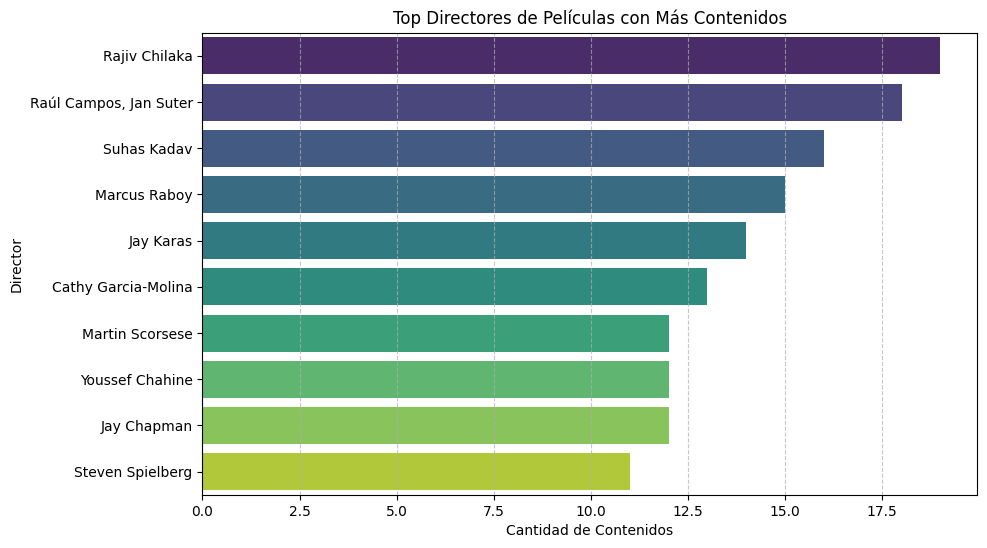
\includegraphics[width=\textwidth]{Graphs/directores_peliculas.png}
    \caption{Directores de Películas Más Comunes}
    \label{fig:peliculas_duracion}
\end{figure}

\begin{figure}[H]
    \centering
    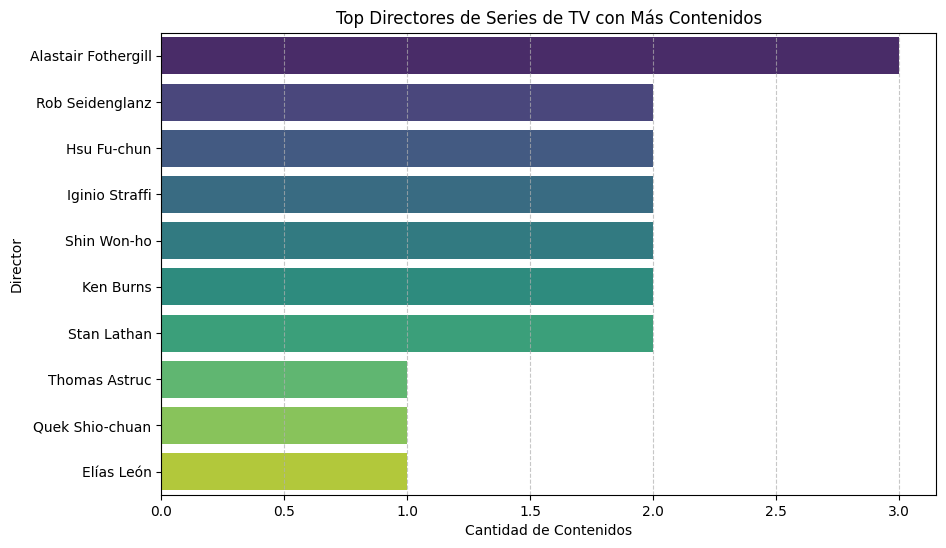
\includegraphics[width=\textwidth]{Graphs/directores_series.png}
    \caption{Directores de Series Más Comunes}
    \label{fig:peliculas_duracion}
\end{figure}

\begin{figure}[H]
    \centering
    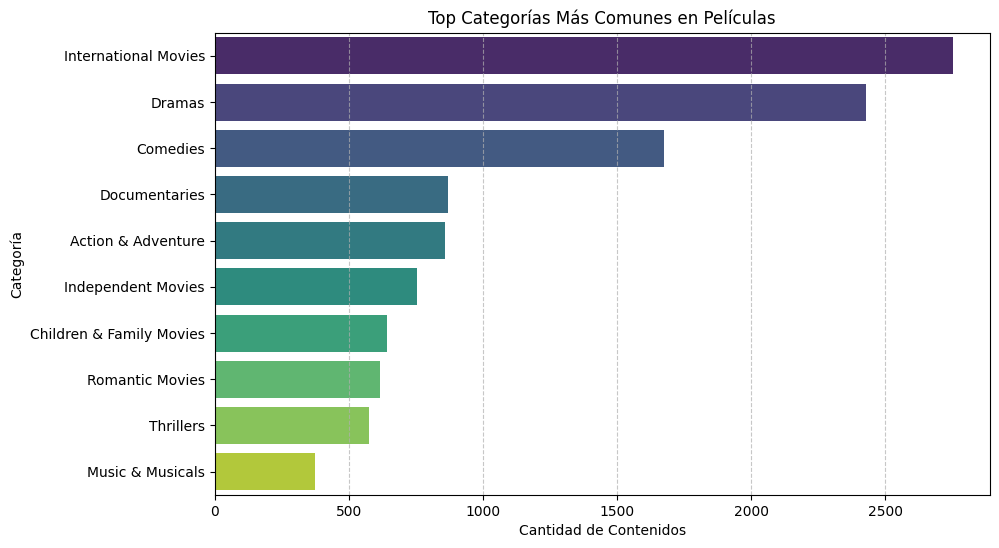
\includegraphics[width=\textwidth]{Graphs/categorias_peliculas.png}
    \caption{Categorías Más Comunes en Películas}
    \label{fig:categorías_peliculas}
\end{figure}

\begin{figure}[H]
    \centering
    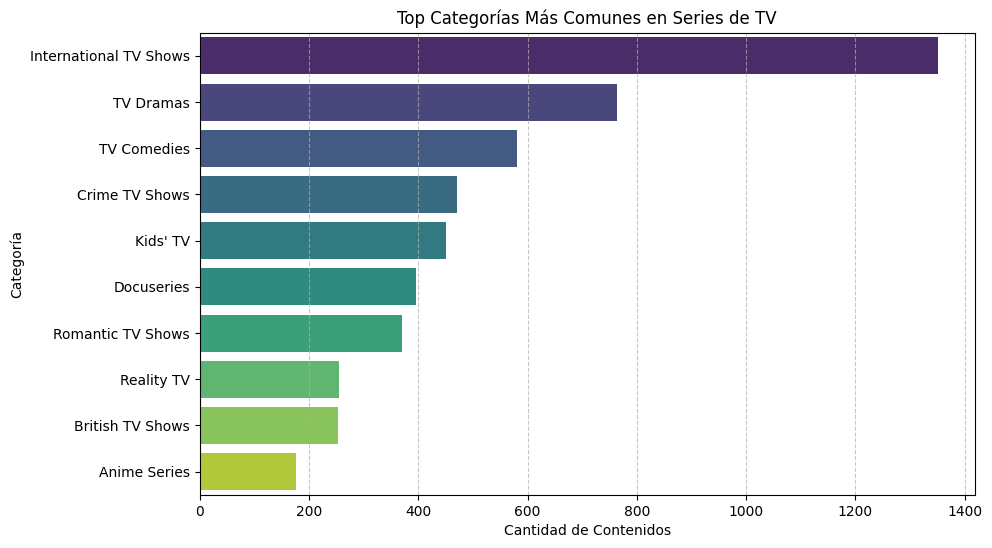
\includegraphics[width=\textwidth]{Graphs/categorias_series.png}
    \caption{Categorías Más Comunes en Series de TV}
    \label{fig:categorías_series}
\end{figure}

\begin{figure}[H]
    \centering
    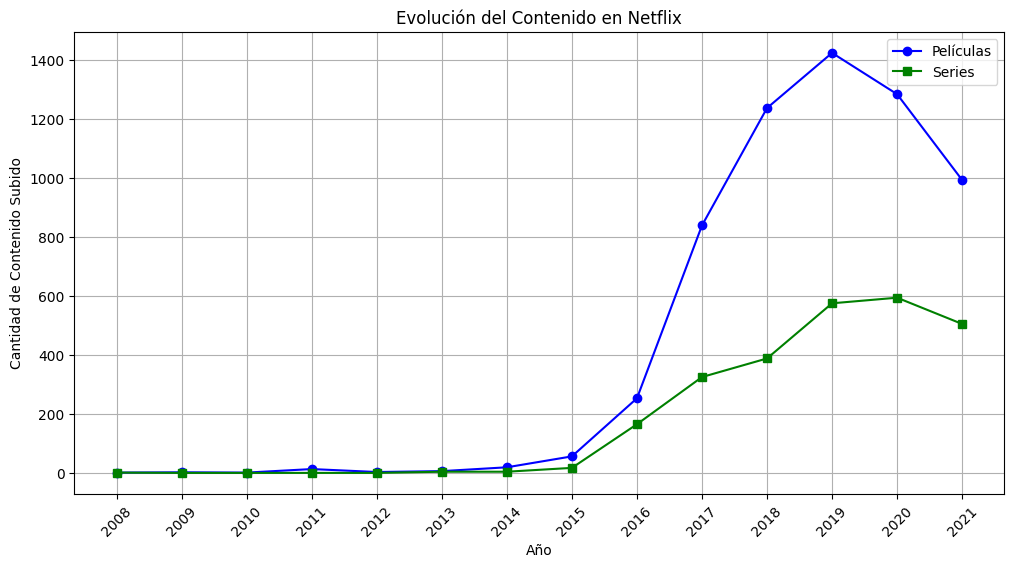
\includegraphics[width=\textwidth]{Graphs/evolucion_contenido.png}
    \caption{Evolución del Contenido}
    \label{fig:evolucion_contenido}
\end{figure}

\begin{figure}[H]
    \centering
    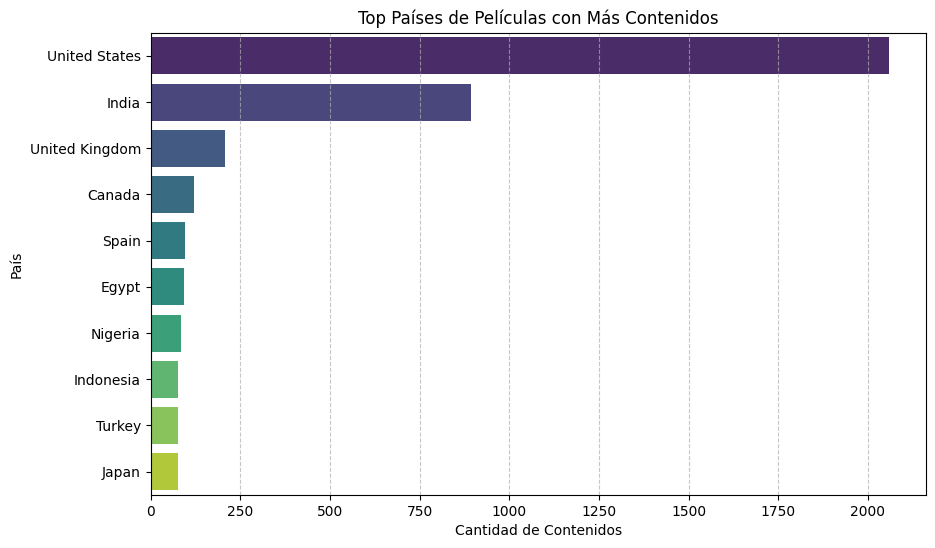
\includegraphics[width=\textwidth]{Graphs/paises_peliculas.png}
    \caption{Países con más películas}
    \label{fig:peliculas_paises}
\end{figure}

\begin{figure}[H]
    \centering
    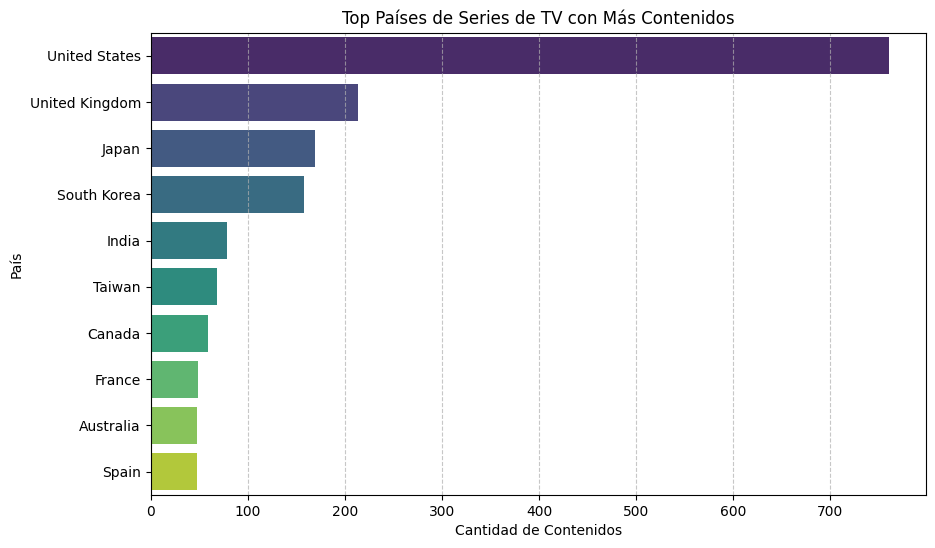
\includegraphics[width=\textwidth]{Graphs/paises_series.png}
    \caption{Países con más series}
    \label{fig:peliculas_paises}
\end{figure}

\begin{figure}[H]
    \centering
    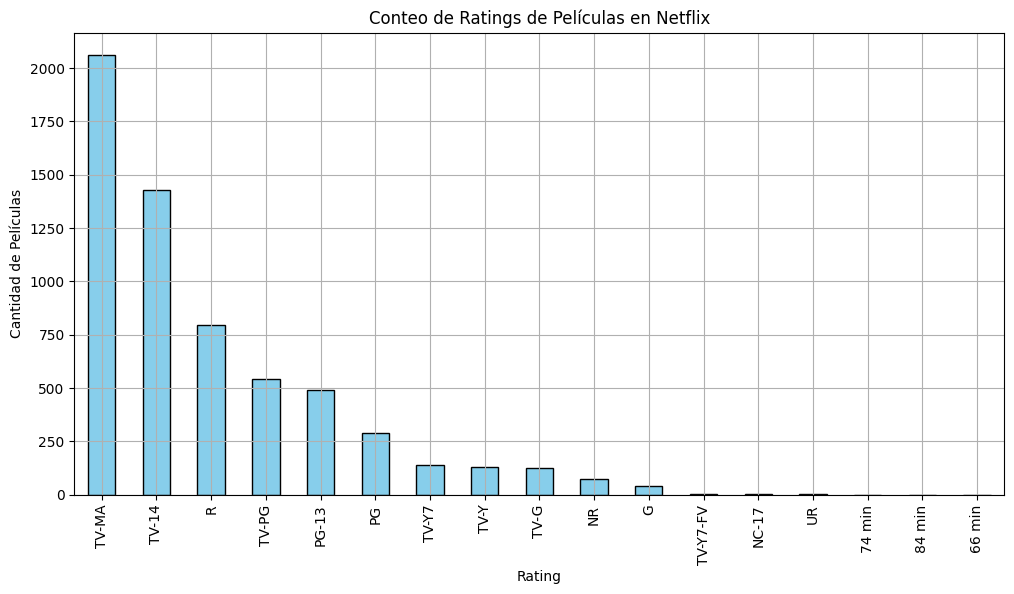
\includegraphics[width=\textwidth]{Graphs/conteo_rating_peliculas.png}
    \caption{Conteo de Ratings para Películas}
    \label{fig:conteo_ratings_peliculas}
\end{figure}

\begin{figure}[H]
    \centering
    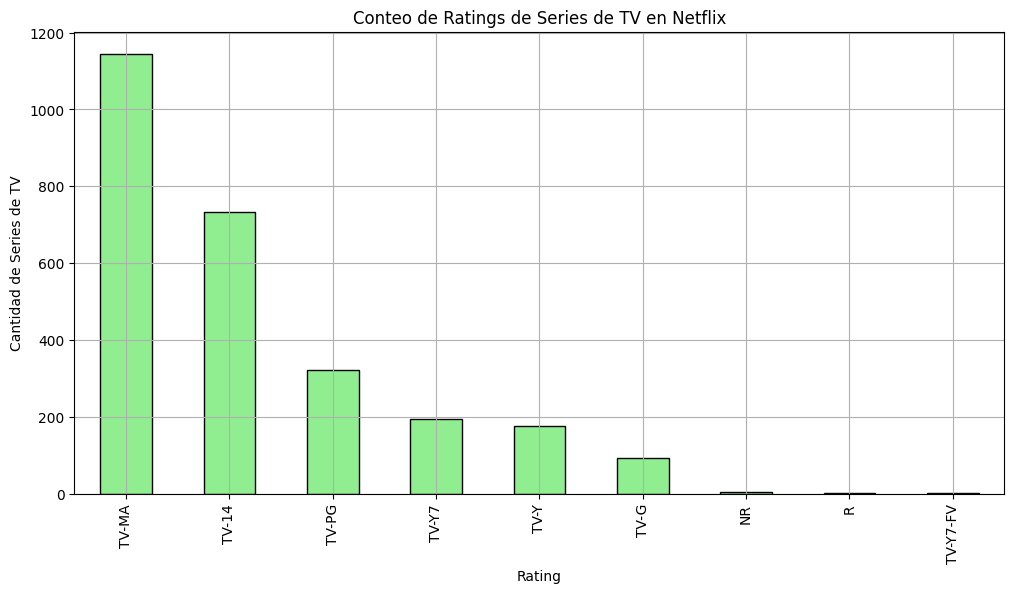
\includegraphics[width=\textwidth]{Graphs/conteo_rating_series.png}
    \caption{Conteo de Ratings para Series de TV}
    \label{fig:conteo_ratings_series}
\end{figure}

\begin{figure}[H]
    \centering
    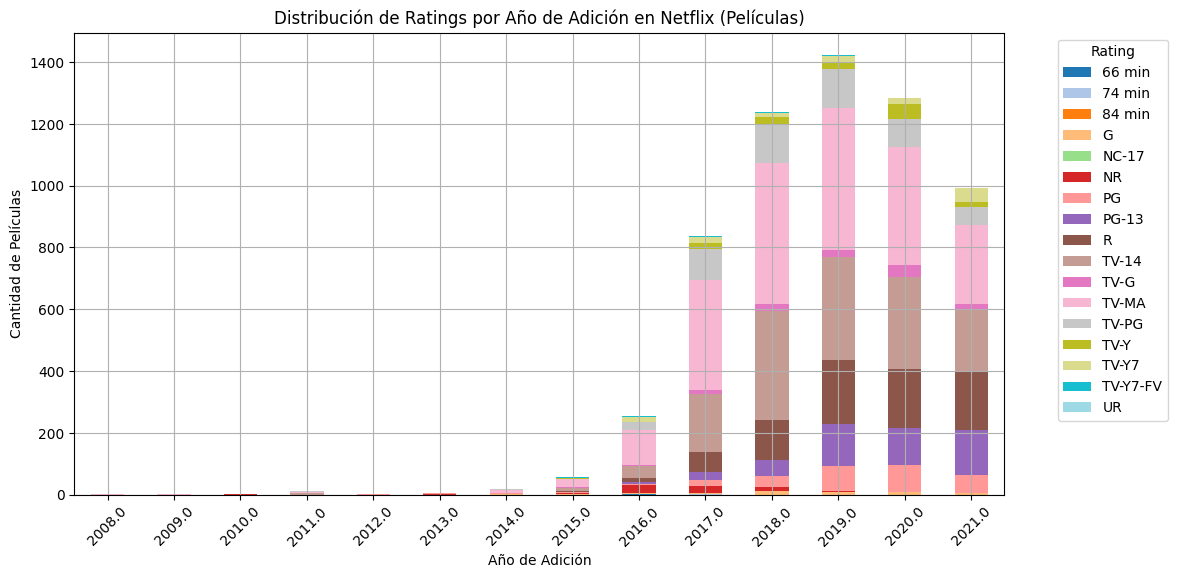
\includegraphics[width=\textwidth]{Graphs/dist_rating_year_peliculas.png}
    \caption{Distribución de Ratings por Año de Adición en Películas}
    \label{fig:distribucion_ratings_peliculas}
\end{figure}

\begin{figure}[H]
    \centering
    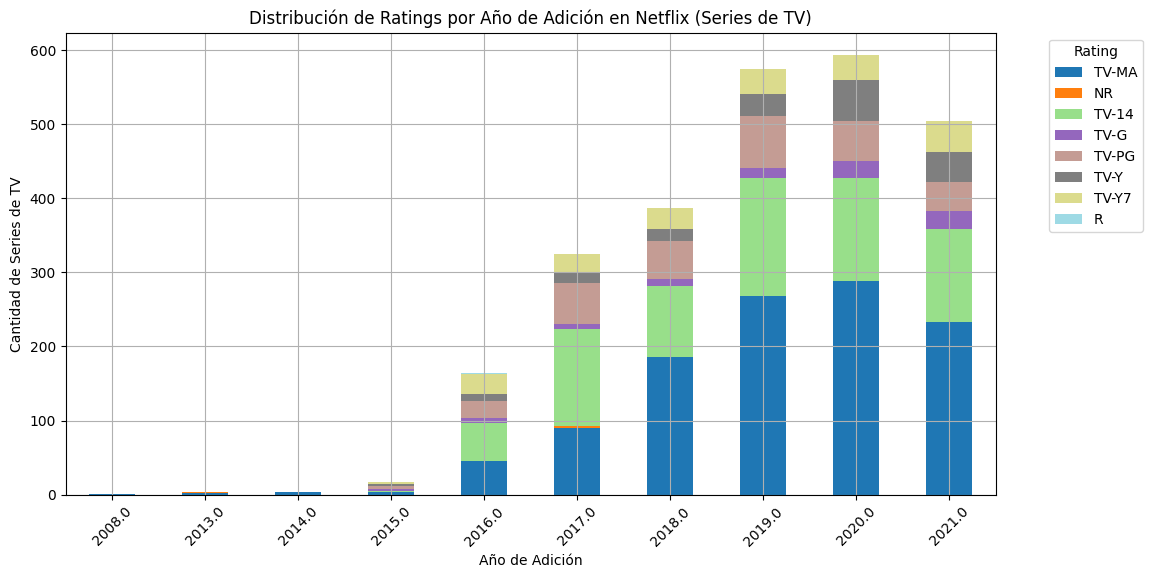
\includegraphics[width=\textwidth]{Graphs/dist_rating_year_series.png}
    \caption{Distribución de Ratings por Año de Adición en Series de TV}
    \label{fig:distribucion_ratings_series}
\end{figure}

\begin{figure}[H]
    \centering
    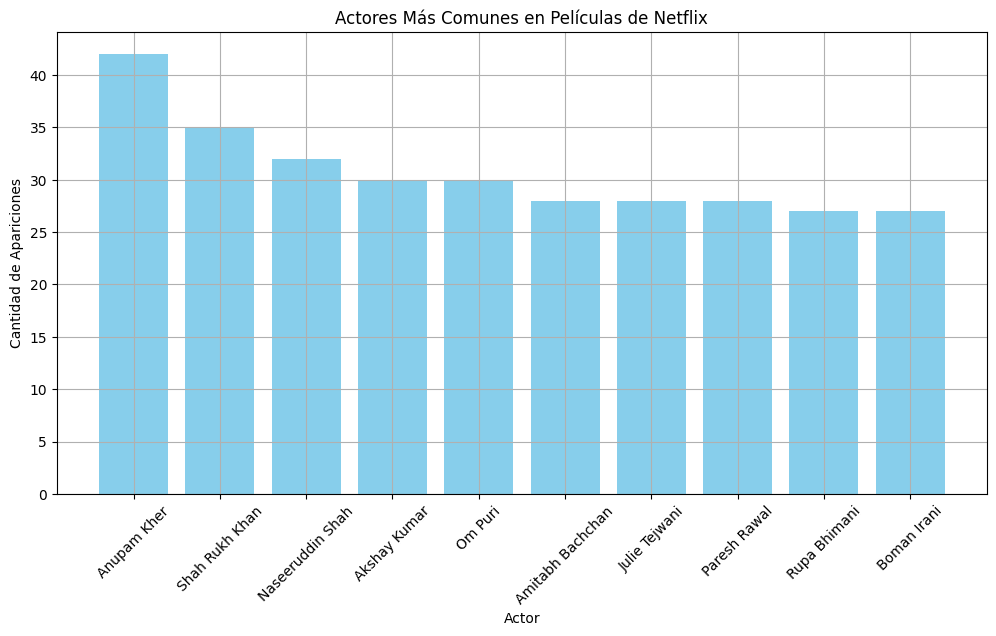
\includegraphics[width=\textwidth]{Graphs/actores_comunes_peliculas.png}
    \caption{Actores Más Comunes en Películas}
    \label{fig:actores_peliculas}
\end{figure}

\begin{figure}[H]
    \centering
    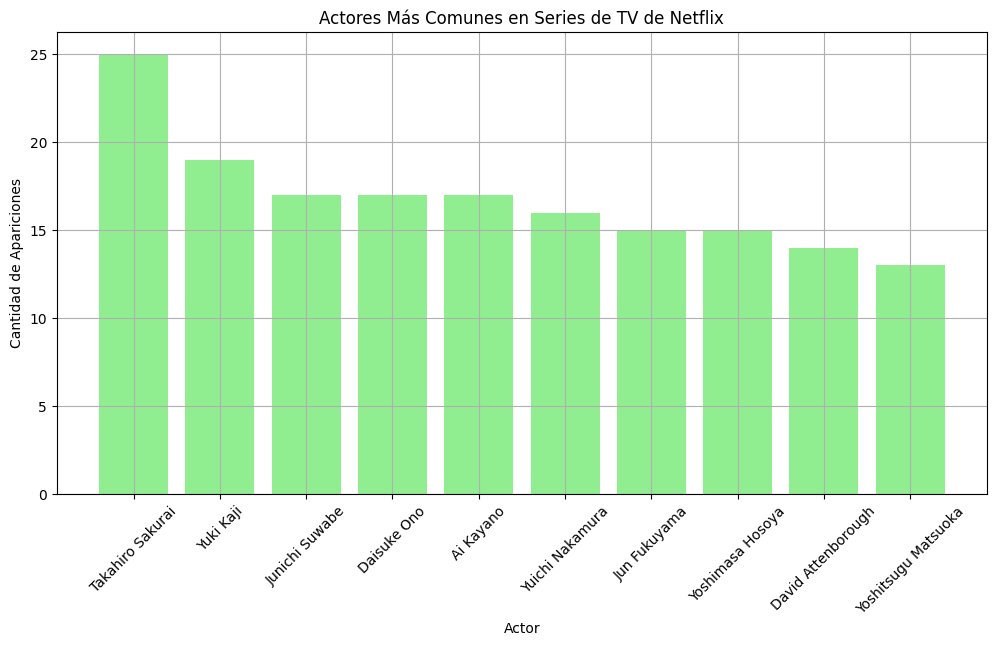
\includegraphics[width=\textwidth]{Graphs/actores_comunes_series.png}
    \caption{Actores Más Comunes en Series de TV}
    \label{fig:actores_series}
\end{figure}

\begin{figure}[H]
    \centering
    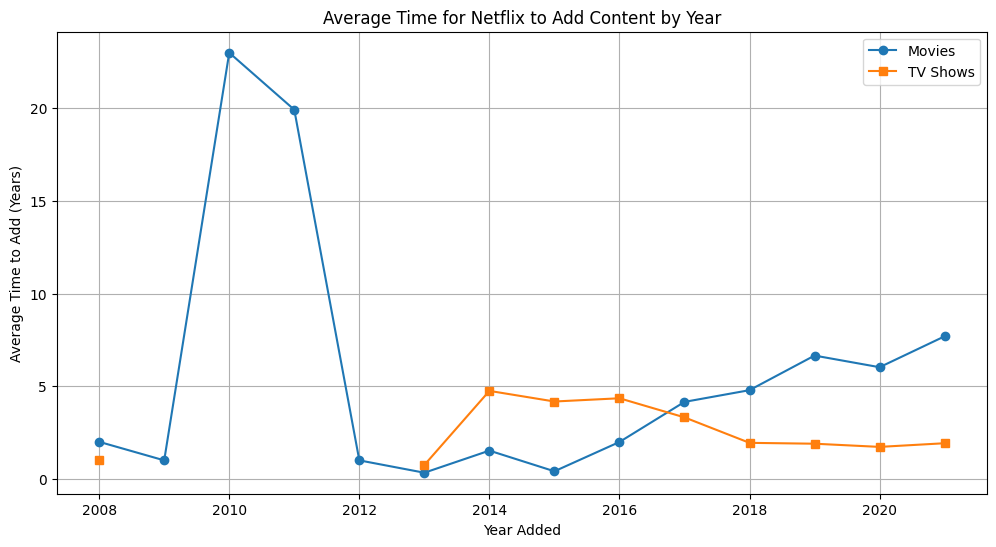
\includegraphics[width=\textwidth]{Graphs/rapidez_adicion.png}
    \caption{Tiempo promedio anual en añadir el contenido a la plataforma desde su estreno }
    \label{fig:rapidez_subida}
\end{figure}

    \subsubsection{Análisis de variables categóricas (tablas de frecuencia, gráficos de barras).}

\subsection{Relaciones Iniciales}
\begin{itemize}
    \item Gráficos de dispersión (scatterplots) para identificar patrones.
    \item Observaciones preliminares sobre tendencias o correlaciones.
\end{itemize}

% --- Sección 3: Análisis de Componentes Principales (PCA) ---
\section{Análisis de Componentes Principales (PCA)}
\subsection{Proceso}
Se realizó un Análisis de Componentes Principales (PCA) para reducir la dimensionalidad del conjunto de datos, que incluye información sobre películas y series de TV. Utilizando seis variables (\textit{tipo, director, duración, fecha de estreno, fecha de adición, rating}), se han codificado las variables categóricas y estandarizado las variables numéricas. Los componentes principales obtenidos (\textit{PC1, PC2, PC3}) capturan la mayor parte de la variabilidad en los datos. Finalmente, se han graficado la varianza explicada por cada componente para visualizar la cantidad de información capturada por cada uno, observando que a partir del segundo componente principal, ya esta se vuelve insignificante.
\subsection{Gráficos}
\begin{figure}[H]
    \centering
    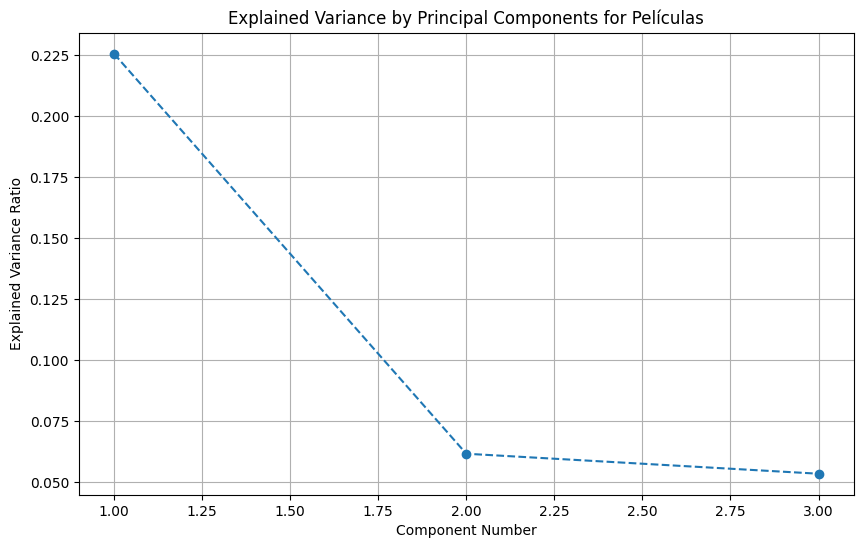
\includegraphics[width=\textwidth]{Graphs/PC_peliculas.png}
    \caption{Varianza explicada por componentes principales (Películas)}
    \label{fig:PC_peliculas}
\end{figure}

\begin{figure}[H]
    \centering
    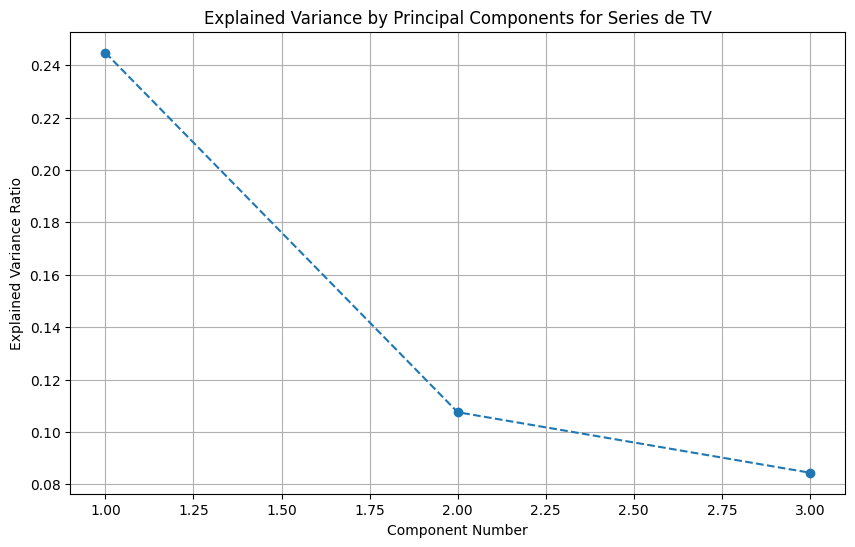
\includegraphics[width=\textwidth]{Graphs/PC_series.png}
    \caption{Varianza explicada por componentes principales (Series)}
    \label{fig:PC_series}
\end{figure}

\begin{figure}[H]
    \centering
    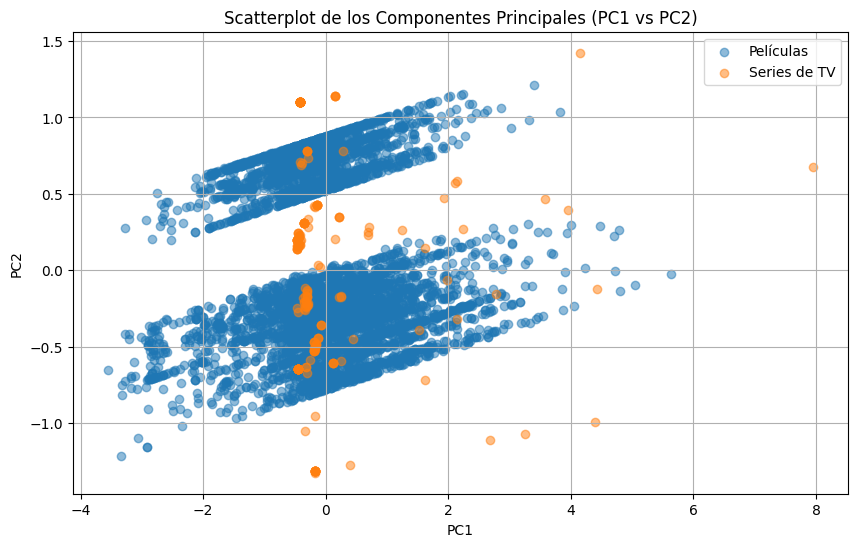
\includegraphics[width=\textwidth]{Graphs/scatterplot.png}
    \caption{Gráfico de puntos para los componentes principales}
    \label{fig:PC_series}
\end{figure}

Dado que el tercer componente principal no captura una porción relativamente influyente de varianza explicada, se ha propuesto hacer el gráfico considerando solo los dos primeros PC. En el caso de las series se da la peculiaridad de que aparece un número anormalmente escaso en dicho gráfico, esto es debido a que no se consideran aquellas que poseen un valor nulo en alguno de los campos correspondientes a las variables que incluimos en el PCA. Esta es una deficiencia del conjunto de datos estudiado.

\section{Test de Normalidad}
En este análisis, se realizó un test de Kolmogorov-Smirnov para evaluar si la muestra de datos sigue una distribución normal. Tras llevar a cabo el test, se concluyó que los datos no siguen una distribución normal, lo cual nos indica que los datos presentan una desviación significativa de la distribución normal teórica.

\begin{figure}[H]
    \centering
    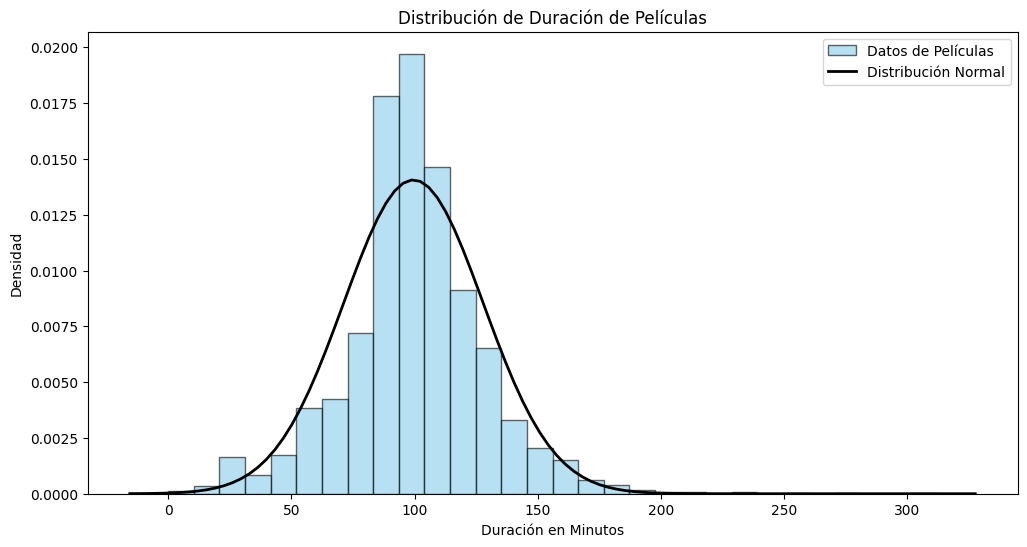
\includegraphics[width=\textwidth]{Graphs/dist_duracion_peliculas.png}
    \caption{Test de normalidad (Peliculas)}
    \label{fig:dist_duracion_peliculas}
\end{figure}

\begin{figure}[H]
    \centering
    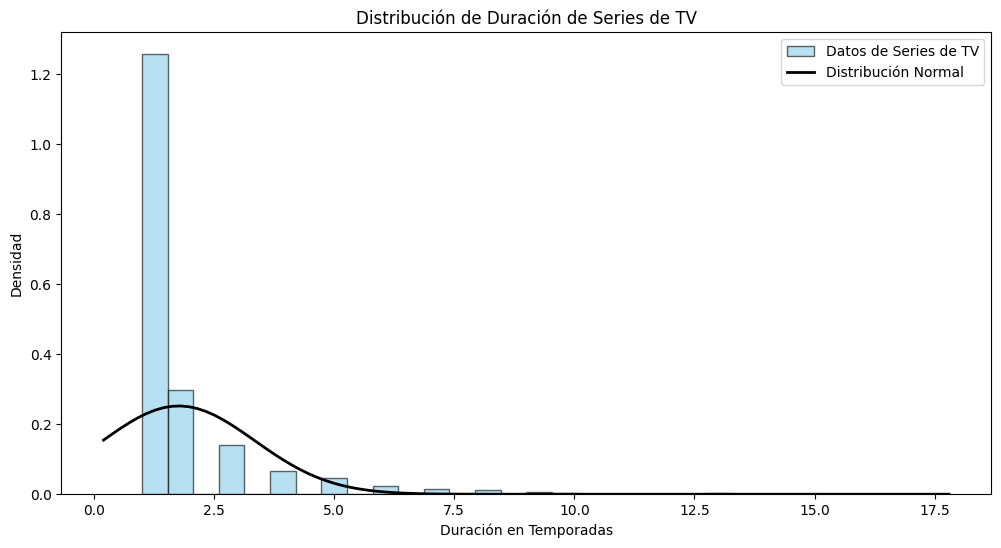
\includegraphics[width=\textwidth]{Graphs/dist_duracion_series.png}
    \caption{Test de normalidad (Series)}
    \label{fig:dist_duracion_series}
\end{figure}



% --- Sección 4: Formulación de Hipótesis ---
\section{Formulación de Hipótesis}
\subsection{Hipótesis Nula y Alternativa}
\begin{itemize}
    \item Hipótesis nula H0 y alternativa H1.
    \item Justificación de las hipótesis basada en el EDA y PCA.
\end{itemize}

\subsection{Pruebas Estadísticas Seleccionadas}
Descripción de las pruebas a utilizar (t-test, ANOVA, chi-cuadrado, etc.) y su relevancia.

% --- Sección 5: Análisis de Correlación ---
\section{Análisis de Correlación}
\subsection{Matriz de Correlación}
\begin{itemize}
    \item Cálculo de la matriz de correlación.
    \item Visualización con heatmap.
\end{itemize}

\subsection{Interpretación de Correlaciones}
\begin{itemize}
    \item Identificación de correlaciones fuertes.
    \item Discusión sobre multicolinealidad y su impacto en el análisis.
\end{itemize}

% --- Sección 6: Regresión Lineal ---
\section{Regresión Lineal}
\subsection{Selección de Variables}
\begin{itemize}
    \item Variables independientes y dependientes seleccionadas.
    \item Justificación de la selección basada en el EDA, PCA y correlación.
\end{itemize}

\subsection{División del Dataset}
\begin{itemize}
    \item Proporción de datos de entrenamiento y prueba (ej. 80\%-20\%).
\end{itemize}

\subsection{Ajuste del Modelo}
\begin{itemize}
    \item Descripción del modelo de regresión lineal ajustado.
    \item Ecuación del modelo.
\end{itemize}

\subsection{Evaluación del Modelo}
\begin{itemize}
    \item Métricas de rendimiento (R², MSE, MAE).
    \item Análisis de residuos (normalidad, homocedasticidad, independencia).
\end{itemize}

\subsection{Interpretación de Resultados}
\begin{itemize}
    \item Impacto de cada variable independiente en la dependiente.
    \item Conclusiones basadas en los coeficientes del modelo.
\end{itemize}

% --- Sección 7: Validación y Conclusiones ---
\section{Validación y Conclusiones}
\subsection{Validación Cruzada}
\begin{itemize}
    \item Descripción del proceso de validación cruzada.
    \item Resultados de la validación.
\end{itemize}

\subsection{Conclusiones}
\begin{itemize}
    \item Resumen de los hallazgos principales.
    \item Limitaciones del análisis.
    \item Recomendaciones basadas en los resultados.
\end{itemize}

% --- Sección 8: Apéndices ---
\section{Apéndices}
\subsection{Código Utilizado}
Incluye el código utilizado para el análisis (si es relevante).

\subsection{Tablas y Figuras Adicionales}
\begin{itemize}
    \item Tablas y gráficos que no se incluyeron en el cuerpo principal pero que son relevantes.
\end{itemize}

% --- Referencias ---
\section*{Referencias}
\begin{itemize}
    \item Libros, artículos o recursos utilizados para el análisis.
\end{itemize}

\end{document}